\documentclass{beamer}
\usepackage[utf8]{inputenc}

\usetheme{Madrid}
\usecolortheme{default}
\usepackage{amsmath,amssymb,amsfonts,amsthm}
\usepackage{txfonts}
\usepackage{tkz-euclide}
\usepackage{listings}
\usepackage{adjustbox}
\usepackage{array}
\usepackage{tabularx}
\usepackage{gvv}
\usepackage{lmodern}
\usepackage{circuitikz}
\usepackage{tikz}
\usepackage{graphicx}

\setbeamertemplate{page number in head/foot}[totalframenumber]

\usepackage{tcolorbox}
\tcbuselibrary{minted,breakable,xparse,skins}



\definecolor{bg}{gray}{0.95}
\DeclareTCBListing{mintedbox}{O{}m!O{}}{%
  breakable=true,
  listing engine=minted,
  listing only,
  minted language=#2,
  minted style=default,
  minted options={%
    linenos,
    gobble=0,
    breaklines=true,
    breakafter=,,
    fontsize=\small,
    numbersep=8pt,
    #1},
  boxsep=0pt,
  left skip=0pt,
  right skip=0pt,
  left=25pt,
  right=0pt,
  top=3pt,
  bottom=3pt,
  arc=5pt,
  leftrule=0pt,
  rightrule=0pt,
  bottomrule=2pt,
  toprule=2pt,
  colback=bg,
  colframe=orange!70,
  enhanced,
  overlay={%
    \begin{tcbclipinterior}
    \fill[orange!20!white] (frame.south west) rectangle ([xshift=20pt]frame.north west);
    \end{tcbclipinterior}},
  #3,
}
\lstset{
    language=C,
    basicstyle=\ttfamily\small,
    keywordstyle=\color{blue},
    stringstyle=\color{orange},
    commentstyle=\color{green!60!black},
    numbers=left,
    numberstyle=\tiny\color{gray},
    breaklines=true,
    showstringspaces=false,
}
%------------------------------------------------------------
%This block of code defines the information to appear in the
%Title page
\title %optional
{1.5.15}
\date{Agust, 2025}
%\subtitle{A short story}

\author % (optional)
{INDHIRESH S - EE25BTECH11027}



\begin{document}


\frame{\titlepage}
\begin{frame}{Question}
The midpoint of the line segment joining $A(2a, 4)$ and $B(-2, 3b)$ is $(1, 2a + 1)$. Findthe values of a and b.
\end{frame}
\begin{frame}{allowframebreaks}
\frametitle{Equation}

    \centering
    
    \label{tab:parameters}
  \begin{align}
\vec{A}= \myvec{2a\\4} , \vec{B}=\myvec{-2\\3b}
\end{align}
Let the midpoint of points A and B be C. where,
\begin{align}
    \vec{C}=\myvec{1\\2a+1}
\end{align}
   
\end{frame}


\begin{frame}{Theoretical Solution}
We know that the midpoint formula for the points A and B is
\begin{align}
    \vec{C}=\frac{\vec{A}+\vec{B}}{2}
    \end{align}
\begin{align}
    \myvec{1\\2a+1}=\frac{\myvec{2a\\4}+\myvec{-2\\3b}}{2}
\end{align}
\begin{align}
    \myvec{1\\2a+1}=\frac{\myvec{2a-2\\4+3b}}{2}
\end{align}
\begin{align}
    \myvec{1\\2a+1}=\myvec{a-1\\2+\frac{3b}{2}}
\end{align}

\end{frame}
\begin{frame}
\frametitle{Theoretical Solution}
From Eq.6 we can say that:
\begin{align}
    2a+1=2+\frac{3b}{2}
\end{align}
\begin{align}
    2a=1+\frac{3b}{2}
\end{align}
\begin{align}
    4a=2+3b
\end{align}
\begin{align}
    4a-3b=2
\end{align}

\end{frame}
\begin{frame}
\frametitle{Theoretical Solution}

Let P=\myvec{C-A& B-A }. A,B and C lies in the same line so they are collinear. So,
\begin{align}
   rank\myvec{C-A&B-A}=1\\
   rank\myvec{1-2a&-2-2a\\
   2a-3&3b-4}=1
\end{align}
Now by applying the row operation for the matrix P\\
$R_2\longrightarrow R_2-(\frac{2a-3}{1-2a})R_1$

\begin{align}
    P=\myvec{1-2a&-2-2a\\0&3b-4-(\frac{2a-3}{1-2a})(-2-2a)}
\end{align}
For the rank to be 1 , all entries of $R_2$ should be zero. so,
\begin{align}
3b-4-(\frac{2a-3}{1-2a})(-2-2a)=0
\end{align}

\end{frame}
\begin{frame}
\frametitle{Theoretical Solution}
\begin{align}
    \frac{(3b-4)(1-2a)+(2a-3)(2+2a)}{1-2a}=0
\end{align}
\begin{align}
    \frac{4a^2-6ab+6a+3b-10}{1-2a}=0
\end{align}
\begin{align}
    4a^2-6ab+6a+3b-10=0
\end{align}

From Eq.10 we can get
\begin{align}
    b=\frac{4a-2}{3}
\end{align}
Now substituting 'b' in Eq.17, we get:
\begin{align}
2a^2-7a+6=0
\end{align}

\end{frame}
\begin{frame}
By solving the above quadratic equation we get:
\begin{align}
a=2,\frac{3}{2}
\end{align}
By substituting the value of 'a' in Eq.18, we get:
\begin{align}
b=2,\frac{4}{3}
\end{align}
But when $a=\frac{3}{2}$ and $b=\frac{4}{3}$ it does not satisfies the Eq.3\\
So the final value of a and b are:
\begin{align}
    a=2\;and\;b=2
\end{align}
\end{frame}


\begin{frame}[fragile]
    \frametitle{C Code - Midpoint formula }

    \begin{lstlisting}
#include <stdio.h>

// Function to calculate midpoint
void midpoint(float x1, float y1, float x2, float y2, float *mx, float *my) {
    *mx = (x1 + x2) / 2.0;
    *my = (y1 + y2) / 2.0;
}


    \end{lstlisting}
\end{frame}


\begin{frame}[fragile]
    \frametitle{Python Code}
    \begin{lstlisting}
import numpy as np
import ctypes
import matplotlib.pyplot as plt

# Load the shared library
lib = ctypes.CDLL("./midpoint.so")   # use "midpoint.dll" on Windows

# Define function signature
lib.midpoint.argtypes = [
    ctypes.c_float, ctypes.c_float,  # x1, y1
    ctypes.c_float, ctypes.c_float,  # x2, y2
    ctypes.POINTER(ctypes.c_float),  # mx
    ctypes.POINTER(ctypes.c_float)   # my
]






    \end{lstlisting}
\end{frame}

\begin{frame}[fragile]
    \frametitle{Python Code}
    \begin{lstlisting}
# Given values from problem
a, b = 2, 2
A = (2*a, 4)   # (4,4)
B = (-2, 3*b)  # (-2,6)

# Prepare variables to hold midpoint
mx, my = ctypes.c_float(), ctypes.c_float()

# Call the C function
lib.midpoint(A[0], A[1], B[0], B[1], ctypes.byref(mx), ctypes.byref(my))
M = (mx.value, my.value)

print(f"Midpoint from C: {M}")





    \end{lstlisting}
\end{frame}

\begin{frame}[fragile]
    \frametitle{Python Code}

    \begin{lstlisting}
# --- Plot ---
plt.figure(figsize=(6,6))
plt.plot([A[0], B[0]], [A[1], B[1]], 'b-', linewidth=2, label='Line AB')

# Scatter points
plt.scatter(*A, color='red', s=100, label=f"A{A}")
plt.scatter(*B, color='green', s=100, label=f"B{B}")
plt.scatter(*M, color='purple', s=120, marker='*', label=f"M{M}")

# Annotate
plt.text(A[0]+0.2, A[1]+0.2, f"A{A}", fontsize=10)
plt.text(B[0]+0.2, B[1]+0.2, f"B{B}", fontsize=10)
plt.text(M[0]+0.2, M[1]+0.2, f"M{M}", fontsize=10, color="purple")


    \end{lstlisting}
\end{frame}
\begin{frame}[fragile]
    \frametitle{Python Code}

    \begin{lstlisting}
# Axes formatting
plt.axhline(0, color='black', linewidth=0.5)
plt.axvline(0, color='black', linewidth=0.5)
plt.grid(True, linestyle="--", alpha=0.6)
plt.legend()
plt.title("Midpoint using C + Python")
plt.xlabel("X-axis")
plt.ylabel("Y-axis")
plt.show()


    \end{lstlisting}
\end{frame}



\begin{frame}{Plot}
    \begin{center}
        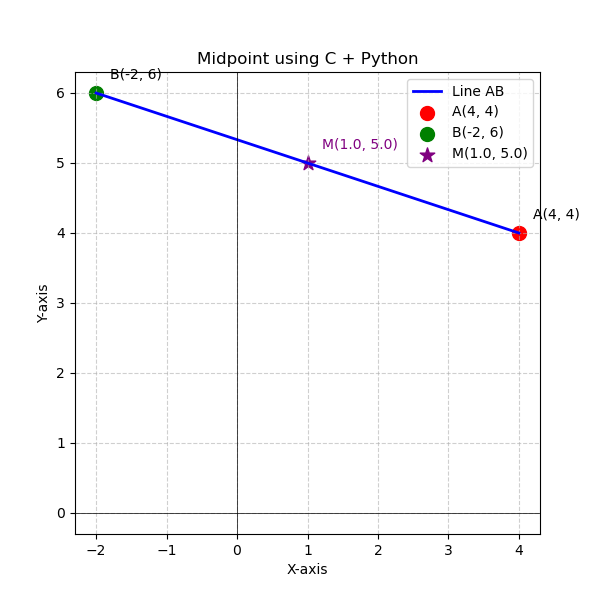
\includegraphics[width=\columnwidth, height=0.8\textheight, keepaspectratio]{figs/figure1.png}
    \end{center}
\end{frame}




\end{document}